\documentclass[12pt,a4paper]{article}
\usepackage{amsmath}
\usepackage{amsfonts}
\usepackage{amssymb}
\usepackage{makeidx}
\usepackage{graphicx}
\usepackage{wrapfig}
\usepackage{enumerate}
\usepackage{pdfpages}
\usepackage{tocloft}
\usepackage{setspace}
\usepackage{mathtools}
\usepackage{hyperref}
\definecolor{linkcolour}{rgb}{0,0.2,0.6} % Link color
\hypersetup{colorlinks,breaklinks,urlcolor=linkcolour,linkcolor=linkcolour}
\usepackage[left=2cm,right=2cm,top=2cm,bottom=2cm]{geometry}

\usepackage{xcolor}
\usepackage{fontspec}
\setmainfont{Cambria}

\usepackage{subcaption}
\usepackage{caption}
\captionsetup[figure]{font=small, labelfont={bf}}
\captionsetup[table]{font=small, labelfont={bf}}

\usepackage{float}
\usepackage{multirow}
\usepackage{longtable}
\usepackage[nottoc]{tocbibind}

\usepackage{soul}

\newcommand{\spa}{\vspace{1.25em}}
\newcommand{\noi}{\noindent}
\def\dul#1{\underline{\underline{#1}}}
\def\cpt#1#2{{\begin{center}\small\textbf{\textcolor{blue}{Figure #1:}} #2\end{center}}}
\def\tt#1{\texttt{#1}}
% for dots in the content
\usepackage{tocloft}
\renewcommand{\cftsecleader}{\cftdotfill{\cftdotsep}}


\begin{document}
    \begin{titlepage} 
        \begin{center}
        \large{ASSIGNMENT 1}\\
        \vspace{2em}
        \large {CS5691 Pattern Recognition and Machine Learning}
        \vspace{3em}
        
        \rule{0.9\linewidth}{0.5mm} \\[0.4cm]
        {\Large{\bfseries{CS5691 Assignemnt 1}}} \\
        \rule{0.9\linewidth}{0.5mm} \\[3 em]    
        
        Team Members: \\
        \vspace{0.5em}
        \def\arraystretch{1.25}
\begin{tabular}{c l}
	\hline
	BE17B007 & N Sowmya Manojna \\
	PH17B010 & Thakkar Riya Anandbhai \\
	PH17B011 & Chaithanya Krishna Moorthy \\
	\hline
\end{tabular}

        \vspace{1em}

        Indian Institute of Technology, Madras\\    
        
        \vspace{5em}    
        
            
\includegraphics[scale = 0.09]{images/iitmlogo.png}
        \end{center}
    \end{titlepage}
{\hypersetup{linkcolor=black}
\tableofcontents}
\break

\section{Task 1}
\subsection{Mathematical Formulation}
The data for univariate polynomial regression is obtained by raising it to the required degree. In case of univariate polynomial regression of degree $d$, the dependent variable, of size $(d,1)$ is assumed to have the form
\begin{equation}
    \vec{y}_{n\times1} = \mathit{\phi}_{n\times d}W_{d\times1}
\end{equation}
\noi
The weights corresponding to a given degree is then calculated by using the closed form solution for univariate polynomial regression:
\begin{equation}
    W = (\mathit{\phi}^T\mathit{\phi} + \lambda \mathit{I})^{-1}\mathit{\phi}^T\vec{y}
\end{equation}
Where, $\lambda\mathit{I}$ is the regularization term.

\subsection{Training and Validation Accuracies}
In order to pick the parameters that best fit the dataset, a grid search was performed on the dataset. Prior to this, the dataset was split into training set, validation set and the testing set, in the ratio 70:10 (from the training data) :30. The results obtained is as follows:
\def\arraystretch{1.25}
\begin{center}
{\small
\begin{longtable}{l l l l l}
\hline
\hline
\textbf{$d$} & \textbf{$\lambda$} & \textbf{Train Error} & \textbf{Validation Error} \\
\hline
\hline
6 & 0.0 & 0.044889 & 0.159636 \\
3 & 0.0 & 0.672882 & 1.001484 \\
9 & 0.5 & 0.750020 & 1.469413 \\
2 & 0.0 & 1.014199 & 1.883134 \\
9 & 1.0 & 1.040132 & 1.929033 \\
9 & 2.0 & 1.354363 & 2.165779 \\
9 & 10.0 & 2.281929 & 1.857270 \\
9 & 50.0 & 3.342110 & 1.447933 \\
9 & 100.0 & 3.782560 & 1.380623 \\
9 & 0.0 & 5.063475 & 92.085167 \\
\hline
\caption{Results obtained for Task 1, with sample size of 10}
\end{longtable}
}
\end{center}

\vspace{-2em}\noi
Regularization was only applied in case of degree 9.\\

\def\arraystretch{1.25}
\begin{longtable}{l l l l l}
\hline
\hline
\textbf{Degree} & \textbf{$\lambda$} & \textbf{Train Error} & \textbf{Validation Error} \\
\hline
\hline
6 & 0.0 & 0.094536 & 0.094379 \\
9 & 0.0 & 0.093581 & 0.100752 \\
9 & 0.5 & 0.134226 & 0.152565 \\
9 & 1.0 & 0.186479 & 0.209008 \\
9 & 2.0 & 0.289107 & 0.311716 \\
9 & 10.0 & 0.766298 & 0.776521 \\
3 & 0.0 & 0.934079 & 0.862605 \\
2 & 0.0 & 1.591842 & 1.421021 \\
9 & 50.0 & 1.620063 & 1.707757 \\
9 & 100.0 & 2.138200 & 2.310223 \\
\hline
\caption{Results obtained for Task 1, with sample size of 200}
\end{longtable}
\noi
\textcolor{blue}{From the table above, we see that the best fit for the data is obtained for degree: $6$ and $\lambda:0$.}

\subsection{Model Fits}
\subsubsection{Sample Size: 10}
The polynomial models and the corresponding fits obtained for sample size of 10 are as follows:
\begin{figure}[H]
    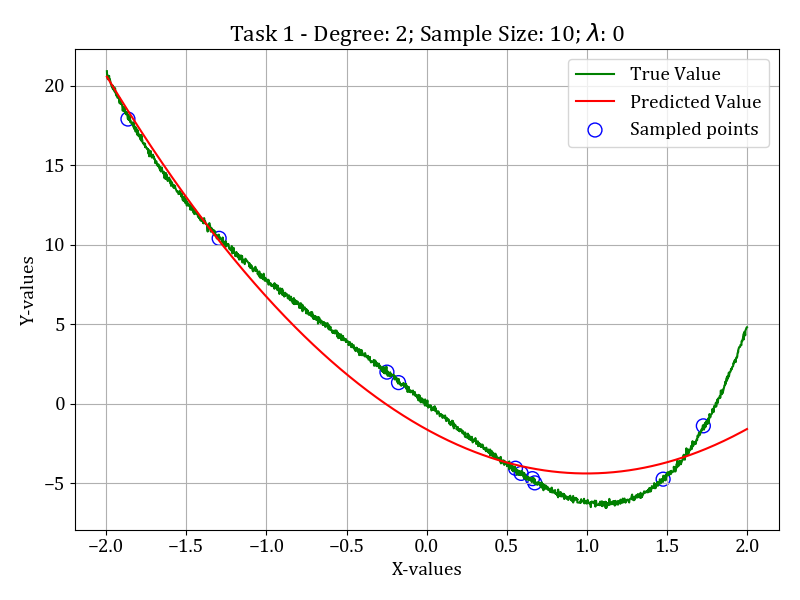
\includegraphics[scale=0.425]{images/t1_d1/d_2_size_10_l_0.png}
    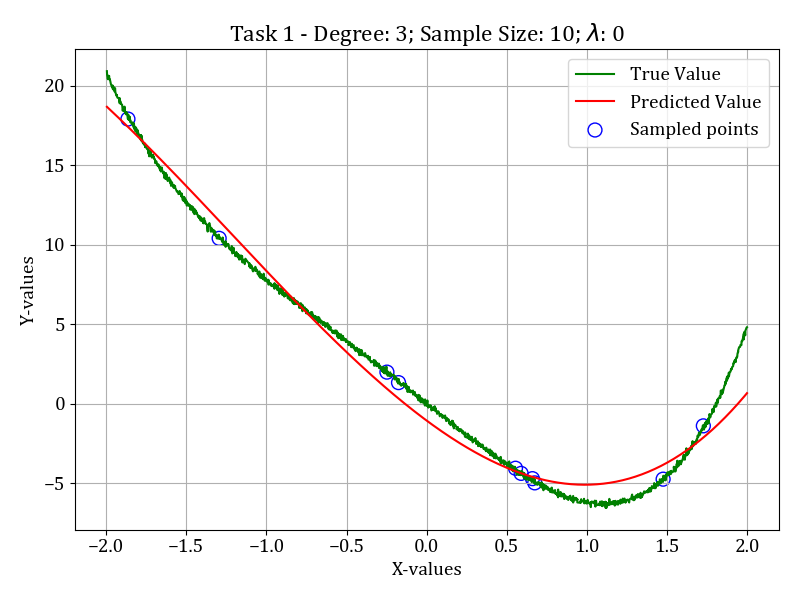
\includegraphics[scale=0.425]{images/t1_d1/d_3_size_10_l_0.png}
    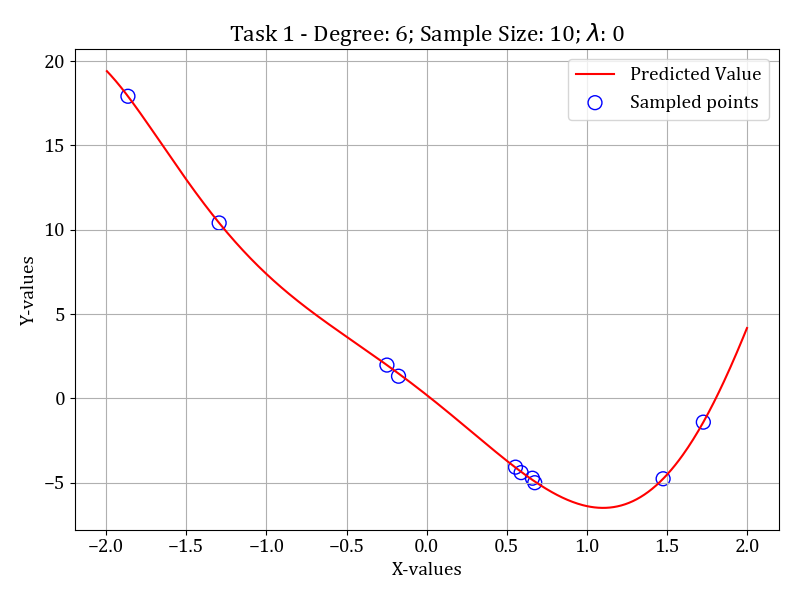
\includegraphics[scale=0.425]{images/t1_d1/d_6_size_10_l_0.png}
    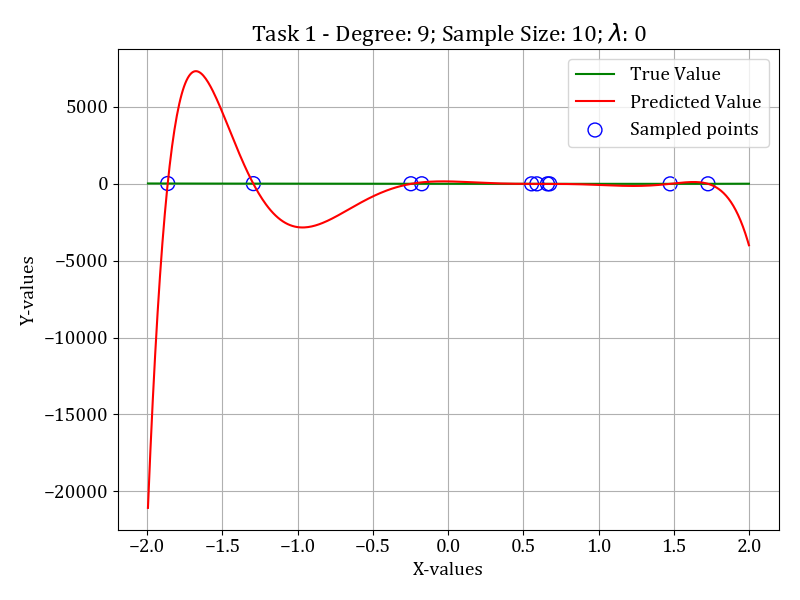
\includegraphics[scale=0.425]{images/t1_d1/d_9_size_10_l_0.png}
    \caption{Task 1 - Polynomial fits, Sample size: 10}
\end{figure}

\subsubsection{Sample Size: 200}
The polynomial models and the corresponding fits obtained for sample size of 200 are as follows:
\begin{figure}[H]
    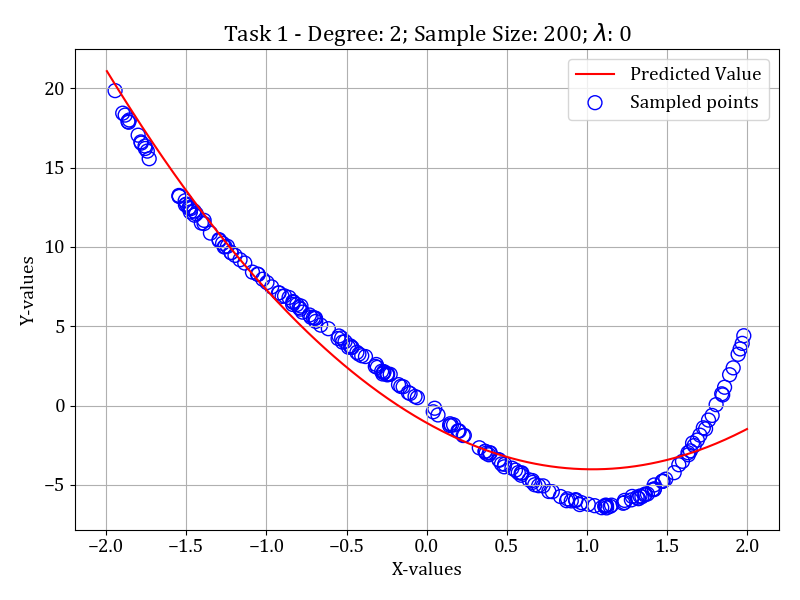
\includegraphics[scale=0.425]{images/t1_d1/d_2_size_200_l_0.png}
    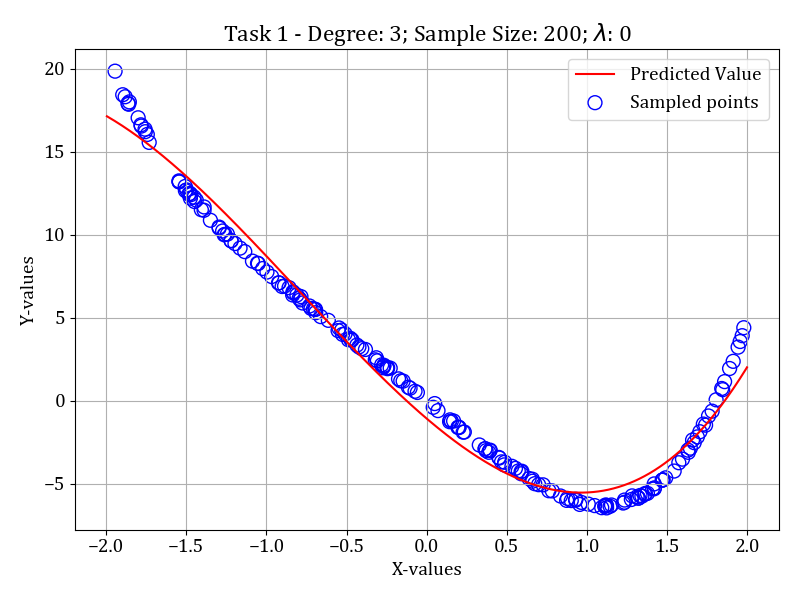
\includegraphics[scale=0.425]{images/t1_d1/d_3_size_200_l_0.png}
    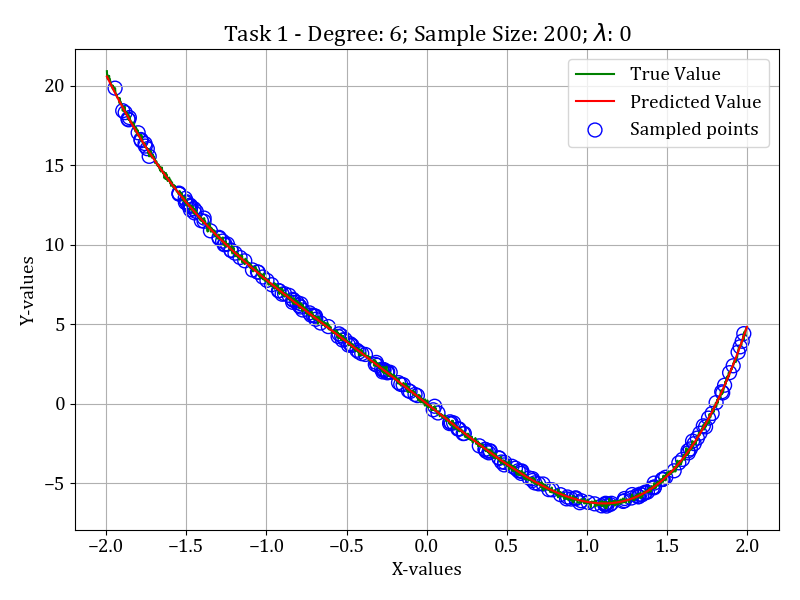
\includegraphics[scale=0.425]{images/t1_d1/d_6_size_200_l_0.png}
    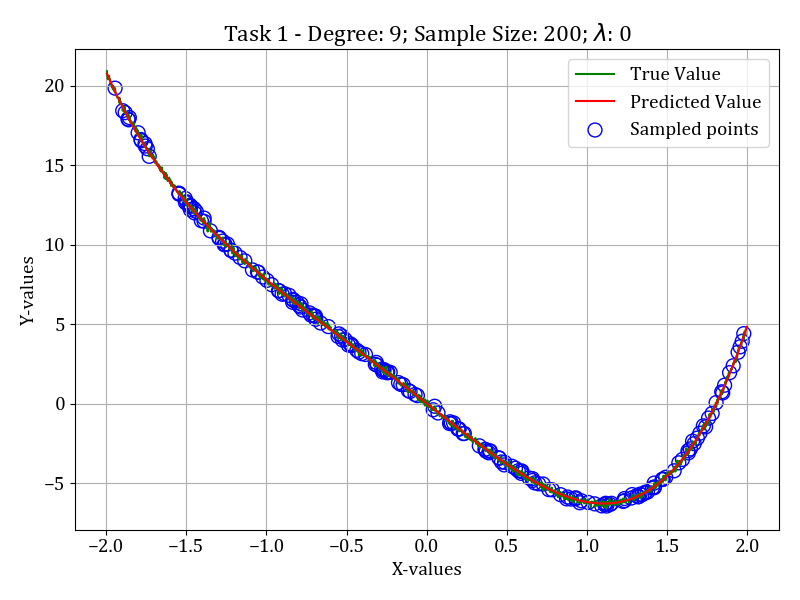
\includegraphics[scale=0.425]{images/t1_d1/d_9_size_200_l_0.png}
    \caption{Task 1 - Polynomial fits, Sample size: 200}
\end{figure}

\subsubsection{Effects of Regularization}
The polynomial models and the corresponding fits obtained for sample size of 10, across different $\lambda$ values are as follows:
\begin{figure}[H]
    \ContinuedFloat
    \begin{subfigure}{\textwidth}
    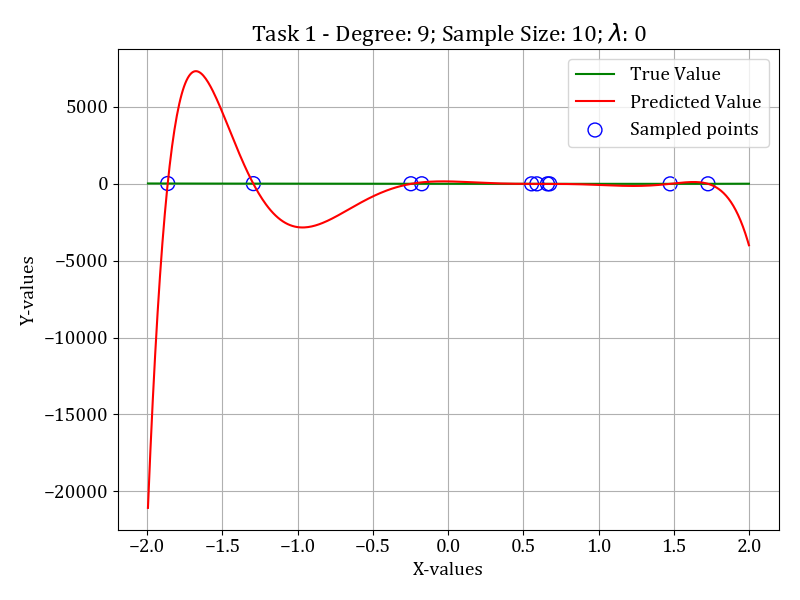
\includegraphics[scale=0.45]{images/t1_d1/d_9_size_10_l_0.png}
    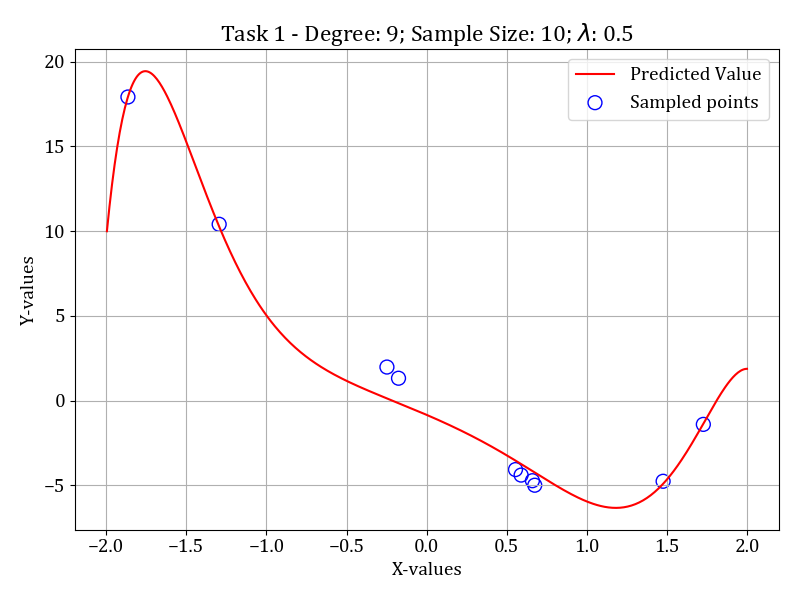
\includegraphics[scale=0.45]{images/t1_d1/d_9_size_10_l_0.5.png}
    \end{subfigure}
    \ContinuedFloat
    \begin{subfigure}{\textwidth}
    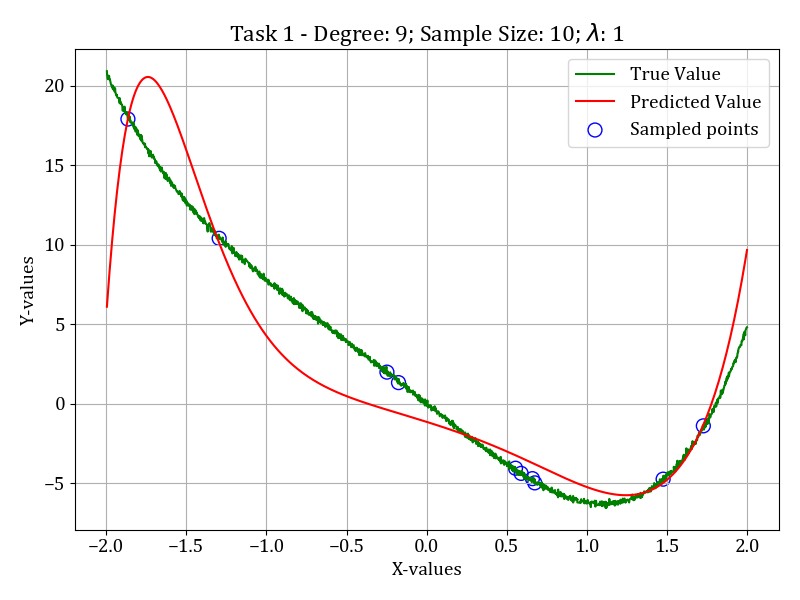
\includegraphics[scale=0.45]{images/t1_d1/d_9_size_10_l_1.png}
    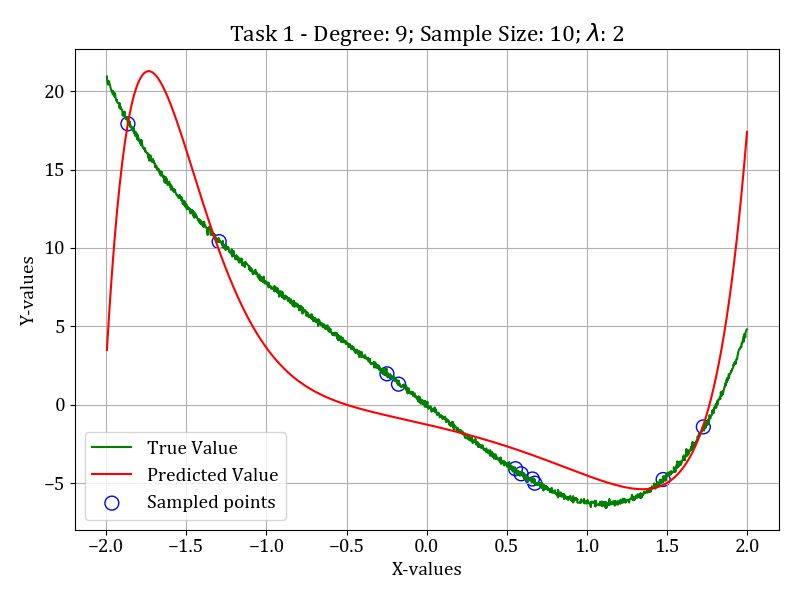
\includegraphics[scale=0.45]{images/t1_d1/d_9_size_10_l_2.png}
    \end{subfigure}
    \ContinuedFloat
    \begin{subfigure}{\textwidth}
    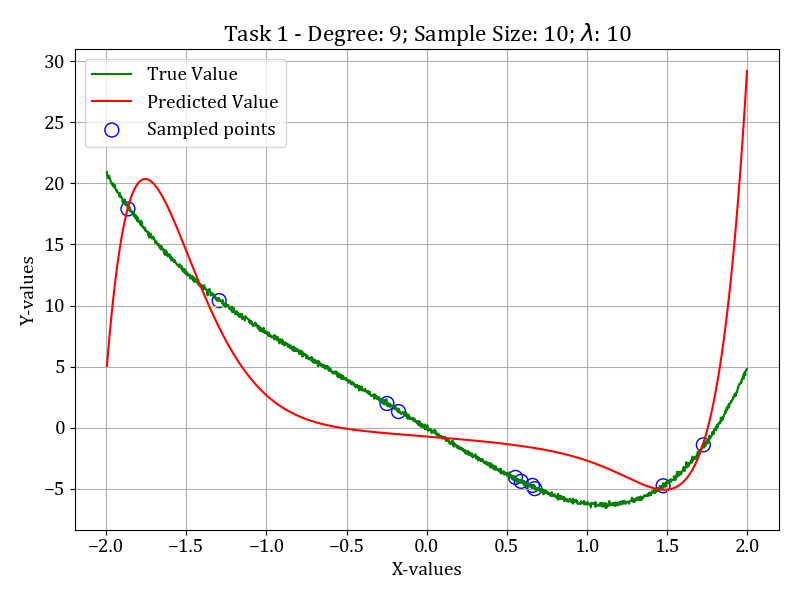
\includegraphics[scale=0.45]{images/t1_d1/d_9_size_10_l_10.png}
    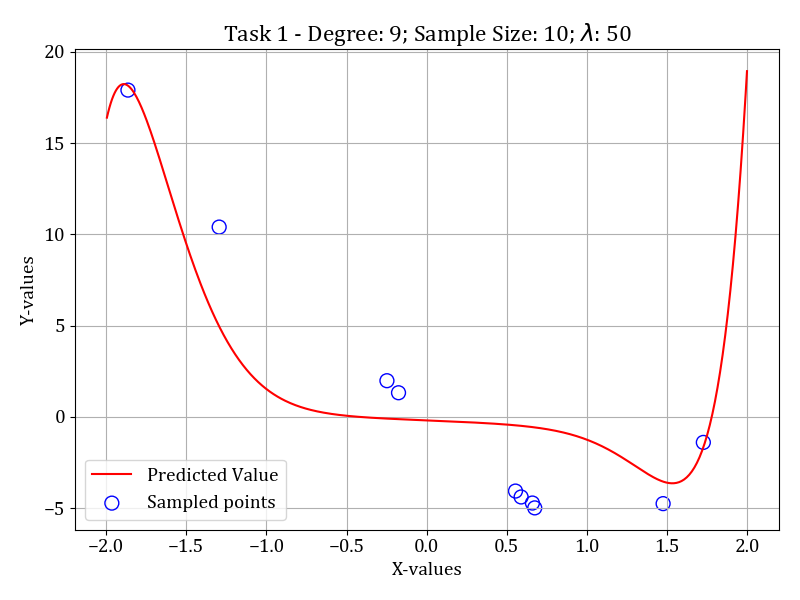
\includegraphics[scale=0.45]{images/t1_d1/d_9_size_10_l_50.png}
    \end{subfigure}
    \ContinuedFloat
    \begin{subfigure}{\textwidth}
    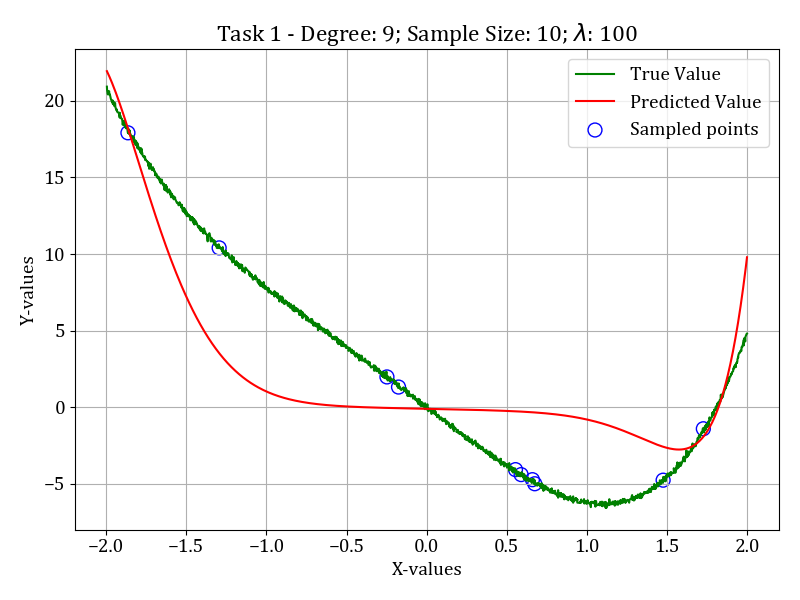
\includegraphics[scale=0.45]{images/t1_d1/d_9_size_10_l_100.png}
    \end{subfigure}
    \caption{Task 1 - 9\textsuperscript{th} Degree Polynomial fit, Sample size: 10}
\end{figure}

\subsection{Best Model}
The best fit, $d:6$ and $\lambda:0$ is visualized as follows:
\begin{figure}[H]
    \centering
    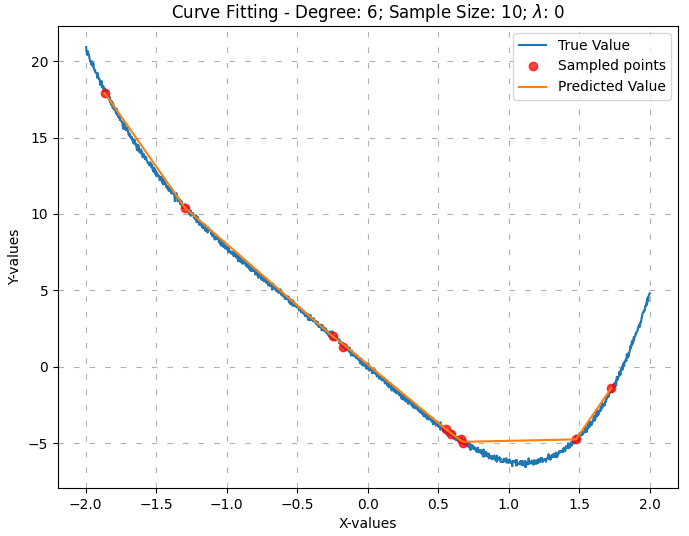
\includegraphics[scale=0.5]{images/d_6_size_10_l_0.png}
    \caption{Task 1 - Best fit, Sample size: 10}
\end{figure}
\begin{figure}[H]
    \centering
    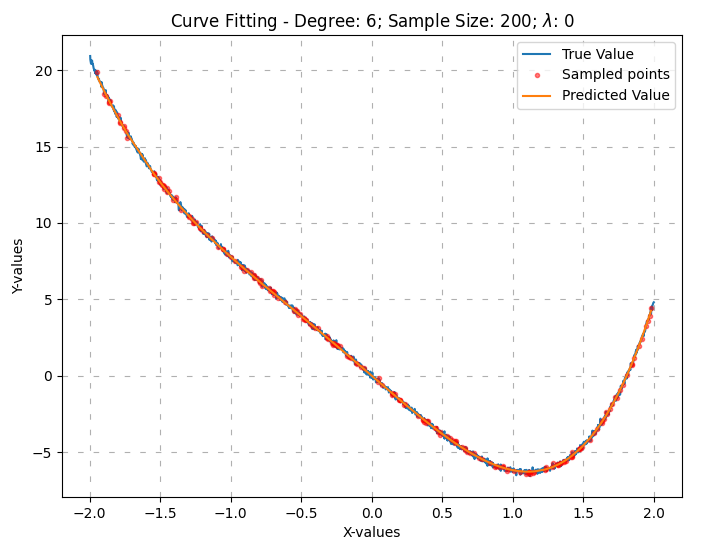
\includegraphics[scale=0.5]{images/d_6_size_200_l_0.png}
    \caption{Task 1 - Best fit, Sample size: 200}
\end{figure}
\noi
The final training and testing error obtained is as follows:
\begin{itemize}
    \itemsep0em
    \item Training Error: 0.09974659089780814
    \item Testing Error: 0.09793071099285168
\end{itemize}

\section{Task 2}

The dataset allotted to our group for task 2 is \tt{function1\_2d.csv}, which has a 2 dimensional feature vector and 1 dimensional target output to be predicted. We assume that the target variable is of the form:
\begin{equation}\label{eq:1}
    y=\sum_{i=0}\omega _{i}\phi_{i}(x1,x2)  +\epsilon 
\end{equation}
Where $\omega_{i}$ are the parameters to be found through regression, $\phi_{i}(x1,x2)$ is a polynomial in x1 and x2 and $\epsilon$ is the normally distributed error. 
\\ A breakdown of the steps undertaken is:

\begin{itemize}
    \item The function \tt{create\_phi} generates the design matrix $\phi(x1,x2)$ for the required degree of complexity.
    The number of attributes in the generated design matrix is given by:
    \begin{equation}
        n=\frac{(d+D)!}{d!\,D!}
    \end{equation}
    where d is the dimension of the original feature vector (=2 for Task 2) and D is the degree of complexity of the model. 
    \item The design matrix is passed to the function \tt{regularized\_pseudo\_inv} , which generates the moore-penrose inverse of the given design matrix(X) and specified value of regularization parameter lambda($\lambda$).
    
    \begin{equation}
         (\lambda I+X^{T}X)^{-1}X^{T}
    \end{equation}
    
    \item The function \tt{opt\_regularized\_param} is then used to obtain optimum values of $\vec{\omega}$
    \begin{equation}
        \vec{\omega} = [(\lambda I+X^{T}X)^{-1}X^{T}].y
    \end{equation}
    Where y is the output as defined in the equation \ref{eq:1}.
    
    \item The optimum parameter vector thus obtained can be used to predict the variable y for new inputs. 
    \begin{equation}
        y_{prediction}=X\vec{\omega}
    \end{equation}
\end{itemize}

The results obtained for various degrees of complexities are discussed below. 

\subsection{Degree of complexity = 2}

With degree of complexity set to 2, the number of parameters in our model are:
\begin{equation}
\begin{split}
 n &= \frac{(d+D)!}{d!\,D!} \\
   & =\frac{(4!)}{2!\,2!} \\
   & =6
\end{split}
\end{equation}
\noi
Since the number of parameters to be estimated is very less compared to our sample sizes, we do not expect to see over fitting, and hence regularisation is not used. 

\subsubsection{Surface plots of Approximated function}

Surface plots obtained for various train sizes are as follows: 
\begin{figure}[H]
    \centering
    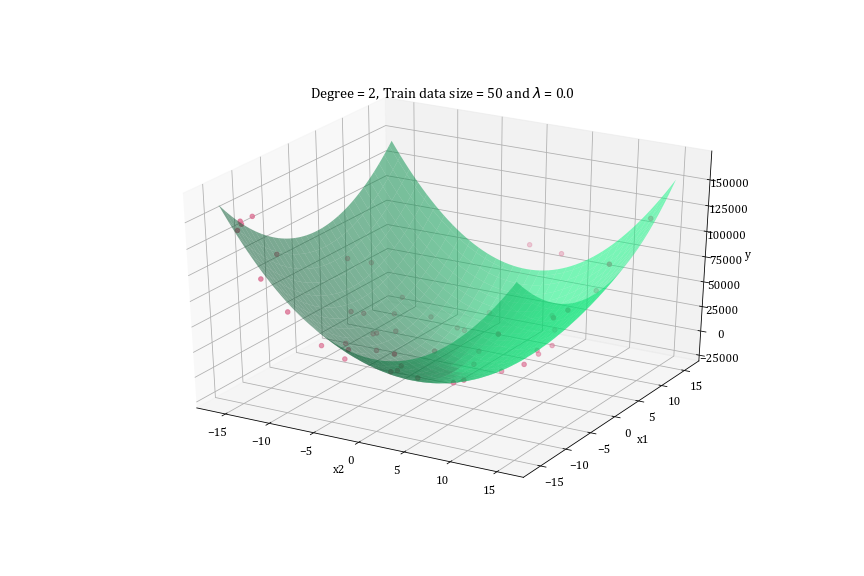
\includegraphics[scale=0.35]{images/D=2,T=50,l=0.0.png}
    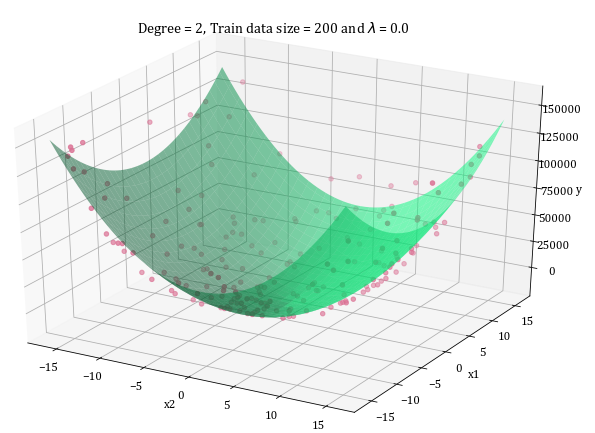
\includegraphics[scale=0.35]{images/D=2,T=200,l=0.0.png}
    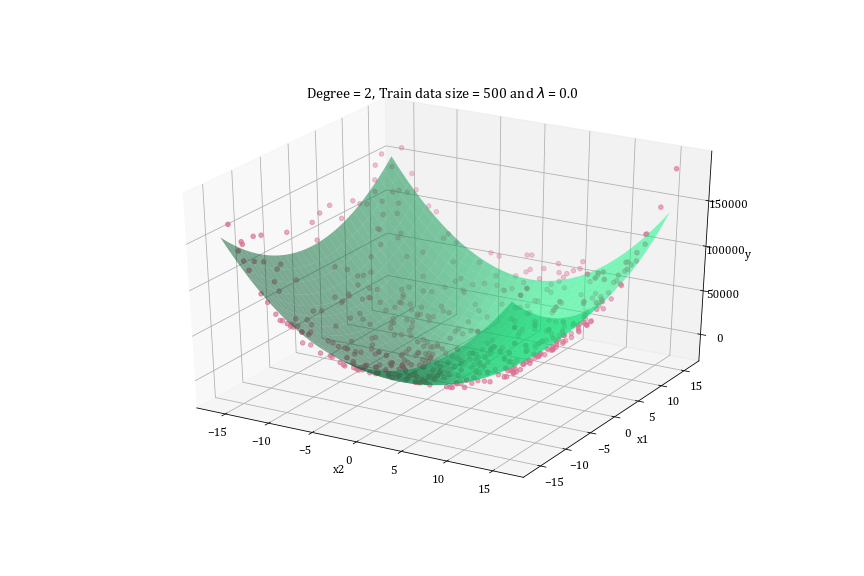
\includegraphics[scale=0.35]{images/D=2,T=500,l=0.0.png}
    \caption{Surface Plot of the approximated function for different training sizes, Degree=2}
    \label{fig:sp_d2}
\end{figure}

\noi

\subsubsection{Erms over Train, Validation and Test data}
The Erms over train, validation and test data is obtained to be: 

\def\arraystretch{1.25}
\begin{table}[H]
\centering
\begin{tabular}{l l l l l}
\hline
\hline
\textbf{Train size} & \textbf{$\lambda$} & \textbf{Erms Train} & \textbf{Erms Validation} & \textbf{Erms Test}\\
\hline
\hline
50 & 0 & 9.34*$10^3$ & 1.06*$10^4$ & 1.14*$10^4$  \\
200 & 0 & 1.06*$10^4$ & 1.14*$10^4$ & 1.15*$ 10^4$  \\
500 & 0 & 1.13*$10^4$ & 1.12*$10^4$ & 1.08*$10^4$\\
\hline
\end{tabular}
\caption{Erms for different train sizes for degree of complexity 2}
\end{table}

\noi
\subsubsection{Observation}
\begin{itemize}
    \item while the magnitude of Erms is nearly same over train, validation and test data, it does not reduce on increasing the sample size. 
    \item The surface plot of approximated function is simple and poorly fits both the training as well as test data.
    \item From the above two points, we conclude that we have an oversimplified model with a high bias. Increasing the complexity would be beneficial.
\end{itemize}

\subsection{Degree of complexity = 3}
The number of parameters to be estimated for this model are: 
\begin{equation}
    \begin{split}
        n&=\frac{(2+3)!}{2!\,3!} \\
         &=10
    \end{split}
\end{equation}
\noi
For this model too, the number of parameters to be estimated are very less compared to the train data sizes, and hence regularization is not required. 

\subsubsection{Surface plots of the approximated function}
The surface plots of approximated function for various train data sizes is: 

\begin{figure}[H]
    \centering
    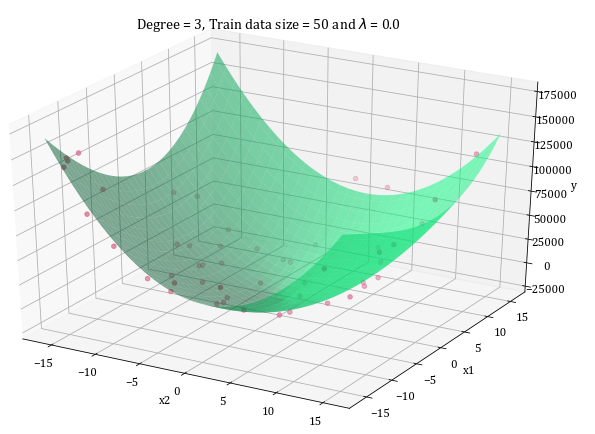
\includegraphics[scale=0.35]{images/D=3,T=50,l=0.0.png}
    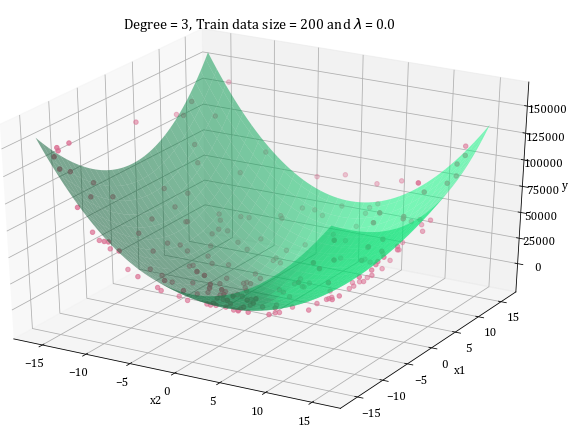
\includegraphics[scale=0.35]{images/D=3,T=200,l=0.0.png}
    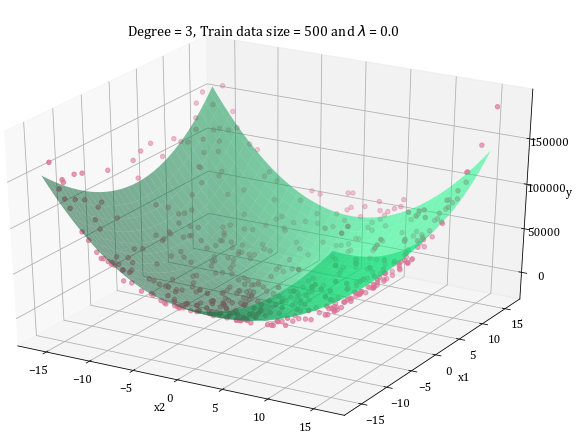
\includegraphics[scale=0.35]{images/D=3,T=500,l=0.0.png}
    \caption{Surface plot of approximated function for different train sizes, Degree=3}
    \label{fig:sp_d3}
\end{figure}

\subsubsection{Erms over Train, Validation and Test data}

The Erms over Train, Validation and Test data is obtained to be:

\def\arraystretch{1.25}
\begin{table}[H]
\centering
\begin{tabular}{l l l l l}
\hline
\hline
\textbf{Train size} & \textbf{$\lambda$} & \textbf{Erms Train} & \textbf{Erms Validation} & \textbf{Erms Test}\\
\hline
\hline
50 & 0 & 8.40*$10^3$ & 1.19*$10^4$ & 1.23*$10^4$  \\
50 & 1 & 8.43*$10^3$ & 1.19*$10^4$ & 1.22*$10^4$ \\
50 & 10 & 9.24*$10^3$ & 1.07*$10^3$ & 1.31*$10^4$ \\
200 & 0 & 1.03*$10^4$ & 1.14*$10^4$ & 1.15*$ 10^4$  \\
500 & 0 & 1.11*$10^4$ & 1.11*$10^4$ & 1.11*$10^4$\\
\hline
\end{tabular}
\caption{Erms for different train sizes for degree of complexity 3}
\end{table}



\subsubsection{Observation}

\begin{itemize}
    \item The Erms values are nearly same as that for degree of complexity 2.
    \item Increasing the sample size does not affect the Erms significantly.
    \item While Erms Train is lower for sample size 50, it is due to inadequate number of data samples. Erms Train, Erms Validation and Erms Test converge as the train data size increases to 500.
    \item From the above points we conclude that this model too is oversimplified and thus fails to perform well over Train, Validation as well as Test data. Our model thus has a high bias error similar to model of complexity 2. 
\end{itemize}

\subsection{Degree of complexity = 6}
The number of parameters to be estimated are-
\begin{equation}
    \begin{split}
        n&=\frac{(2+6)!}{2!\,6!} \\
        &=28
    \end{split}
\end{equation}

\noi
For this model too, the number of parameters to be estimated is far less compared to train data size of 200 and 500. However, for the train data size of 50, we expect a poor estimation of the parameters since the model will not have enough data points. 

\subsubsection{Surface plots of the approximated function}

The surface plots of the approximated function for various train data sizes are:

\begin{figure}[H]
    \centering
    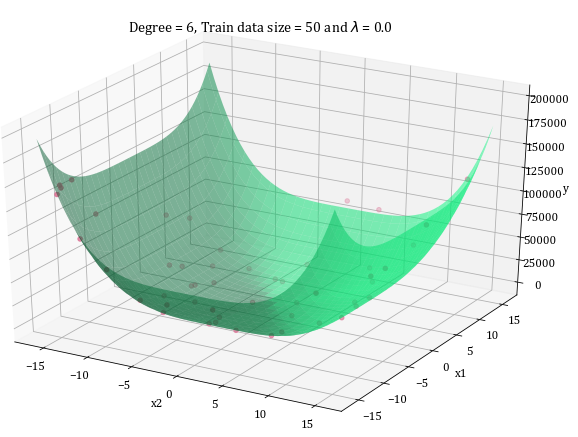
\includegraphics[scale=0.35]{images/D=6,T=50,l=0.0.png}
    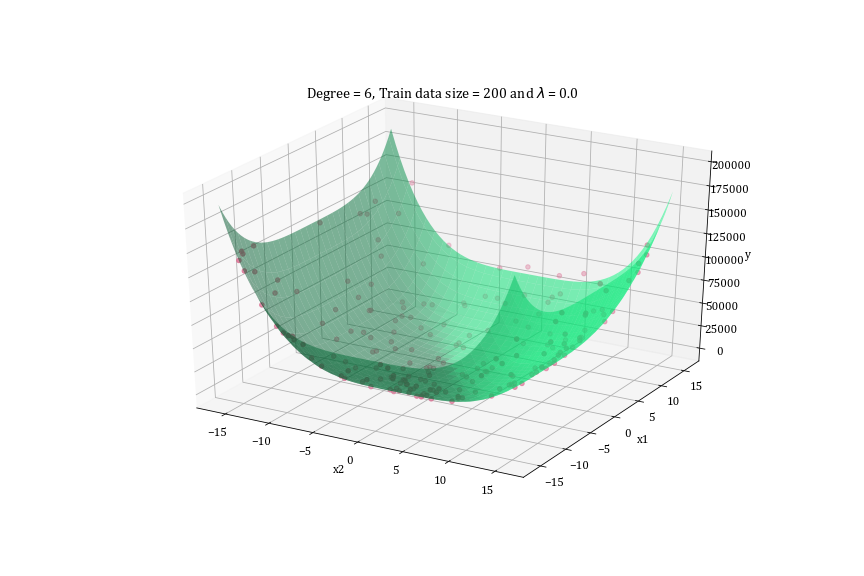
\includegraphics[scale=0.35]{images/D=6,T=200,l=0.0.png}
    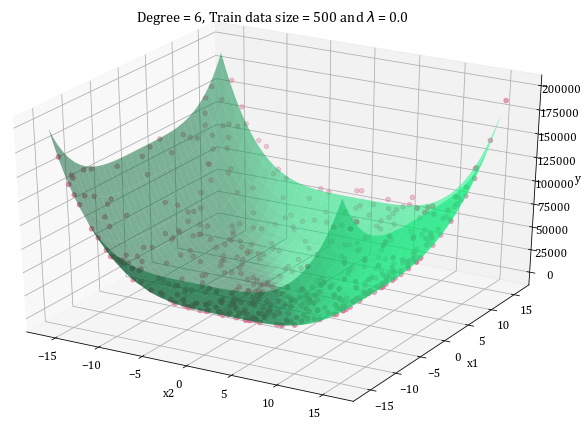
\includegraphics[scale=0.35]{images/D=6,T=500,l=0.0.png}
    \caption{Surface plots of approximated function for different train size, Degree = 6}
    \label{fig:sp_d6}
\end{figure}

\subsubsection{Erms over Train, Validation and Test data}
The Erms values obtained over Train, Validation and Test data are as follows: 
\break

\begin{table}[H]
\centering
\begin{tabular}{l l l l l}
\hline
\hline
\textbf{Train size} & \textbf{$\lambda$} & \textbf{Erms Train} & \textbf{Erms Validation} & \textbf{Erms Test}\\
\hline
\hline
50 & 0 & 7.78*$10^{-8}$ & 3.72*$10^{-7}$ & 6.17*$10^{-7}$  \\
50 & 1 & 1.02*$10^{-4}$ & 1.25*$10^{-3}$ & 2.27*$10^{-3}$ \\
200 & 0 & 1.31*$10^{-8}$ & 1.39*$10^{-8}$ & 1.44*$ 10^{-8}$  \\
500 & 0 & 3.47*$10^{-8}$ & 3.66*$10^{-8}$ & 3.39*$10^{-8}$\\
\hline
\end{tabular}
\caption{Erms for different train sizes for degree of complexity 6}
\end{table}



\subsubsection{Observations}
\begin{itemize}
    \item The complexity of surface in figure \ref{fig:sp_d6} has increased significantly compared to that in figure \ref{fig:sp_d2} and figure \ref{fig:sp_d3}
    \item The Erms values over all the data sets has decreased drastically as compared to the previous models.
    \item While the Erms train is less compared to Erms Validation and Erms Test for train data size = 50, increasing the training data size alleviates this. 
    \item On increasing the train data size to 200, Erms over Train, Validation and Test data all converge to a lower value, signifying an optimum trade off between bias and variance error. Regularization is therefore not required.
    \item On further increasing the Train data size, the Erms increases insignificantly. 
    \item From the above points and cross-validation method, we conclude that the degree of complexity 6 and Train data size of 200 is the optimal model to describe our data, achieving an upper bound Root Mean Squared Error of $~1.5*10^{-8}$ over Train, Validation as well as Test data.
    \item None of the models need to be regularized. On applying regularization, even for very small values of the hyperparameter $\lambda$, the Erms errors increase. 
\end{itemize}

\subsection{Scatter plot of Model output vs Target output}

Using the optimal model of degree 6 and train data size 200, model output vs target output was plotted for both Train and Test data, we find it to closely follow $y-x=0$ line.
\begin{figure}[H]
    \centering
    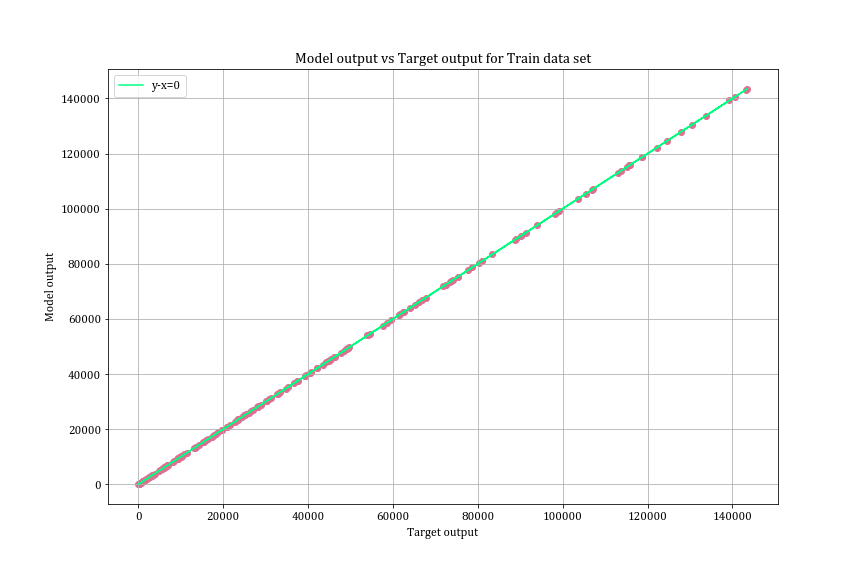
\includegraphics[scale=0.25]{images/tvsy_train.png}
    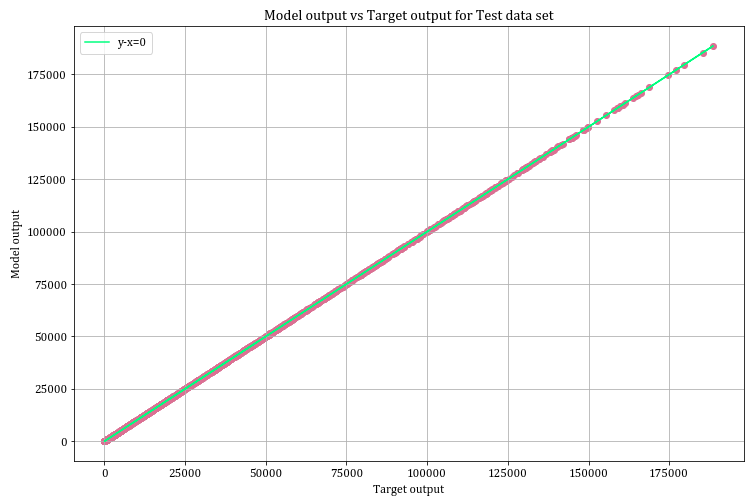
\includegraphics[scale=0.25]{images/tvsy_test.png}
    \caption{Model output vs Target output for train(left) and test dataset(right)}
    \label{fig:yvst}
\end{figure}

\break

\section{Task 3}
Linear regression using Gaussian basis function is given as 
\begin{equation}
    y(\vec{x},\vec{w}) = \sum_{i=0}^{D-1} \omega_{i}\phi_{i}(\vec{x})
\end{equation},
where D is a hyperparameter. The basis function 
\begin{equation}
    \phi_{i} = \exp\Big(\frac{-|\vec{x} - \vec{\mu}_i|^2}{\sigma^2}\Big)
\end{equation}
where $i = 1,2 ... D-1$. The $\mu$ are the mean vectors for $D-1$ kernels made from the data set. The value of the mean vectors are found using the KMeans clustering algorithm. In this work, the \tt{sklearn} KMeans function was used. The optimum number of clusters for the dataset 2 - "\texttt{function\_12d.csv}" was found to be 10 clusters. For the dataset 3 - "\tt{1\_bias\_clean.csv}", the optimum number of clusters are 9.

\subsection{No regularization}
The following plots were obtained:
\begin{figure}[H]
     \centering
     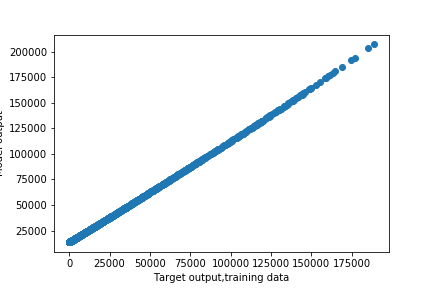
\includegraphics[scale=0.5]{images/scatter_ds2noreg.png}
     \caption{Scatter plot of the target values vs model prediction for Training set of Dataset 2, using linear regression with gaussian basis and no Regularization, $\lambda = 0.01 $}
     \label{fig:ds2tr}
\end{figure}
\begin{figure}[H]
    \centering
    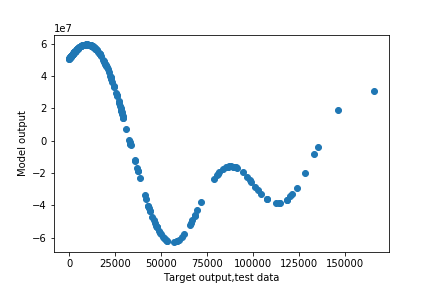
\includegraphics[scale=0.5]{images/scatter_ds2noreg_test.png}
    \caption{Scatter plot of the target values vs model prediction for Test set of Dataset 2, using linear regression with gaussian basis and no Regularization, $\lambda = 0.01 $}
    \label{fig:tikhds2tr}
\end{figure}


\subsection{Quadratic Regularization}
Optimal parameters using quadratic regularization is given by $\vec{\omega^*}$ = $(\Phi^T\Phi + \lambda I)^{-1} \Phi^T \vec{t}$;\\

\noi
$\lambda$ is the regularization parameter. The values $0.01, 0.1,  1.0, 5.0, 10.0$ were used to estimate the optimal parameters and the RMSE on the cross-validation set was calculated for each value. The best performing model was selected as the one having least RMSE on CV data \\

\noi
For dataset 2, the RMSE values for the Training, CV and Test data across $\lambda$ values is:
\def\arraystretch{1.25}
\begin{table}[H]
\centering
\begin{tabular}{l l l l}
\hline
\hline
\textbf{Lambda} & \textbf{RMSE Train} & \textbf{RMSE CV} & \textbf{RMSE Test} \\
\hline
\hline
0.01 & 3059.2231939706166 & 304419.6502059433 & 1309688.1097631603 \\
0.1 & 2967.5181829927037 & 1260.488802049498 & 41195.93571016699 \\
1.0 & 2990.3948869258456 & 1425.9232970077237 & 39596.78510421749 \\
5.0 & 3013.546633117982 & 1503.9615829712025 & 39006.81341800579 \\
10.0 & 3036.360553338793 & 1541.3504903884834 & 38684.11470986189 \\
\hline
\end{tabular}
\captionof{table}{Results obtained for Task 3}
\end{table}


\noi
Scatter plots of the model prediction using the regularization parameter value 0.01:
\begin{figure}[H]
     \centering
     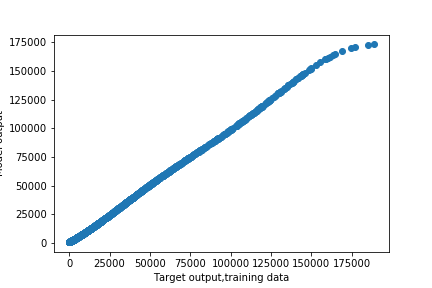
\includegraphics[scale=0.5]{images/scatter_ds2quad.png}
     \caption{Scatter plot of the target values vs model prediction for Training set of Dataset 2, using linear regression with gaussian basis and quadratic Regularization, $\lambda = 0.01 $}
     \label{fig:tikhds2tr}
\end{figure}
\begin{figure}[H]
     \centering
     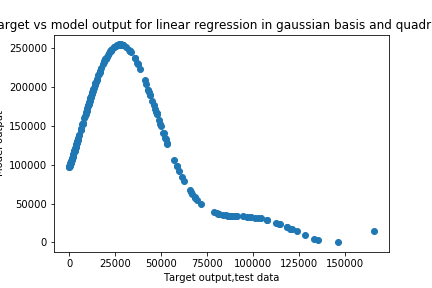
\includegraphics[scale=0.5]{images/scatter_ds2quadtest.png}
     \caption{Scatter plot of the target values vs model prediction for Test set of Dataset 2, using linear regression with gaussian basis and quadratic Regularization, $\lambda = 0.01 $}
     \label{fig:tikhds2tr}
\end{figure}
For dataset 3, the following RMSE table was obtained:
\def\arraystretch{1.25}
\begin{center}
\begin{longtable}{l l l l}
\hline
\hline
\textbf{Lambda} & \textbf{RMSE Train} & \textbf{RMSE CV} & \textbf{RMSE Test} \\
\hline
\hline
0.01 & 4929.01653053444 & 414848.3042013735 & 3312196.0992440097 \\
0.1 & 4624.091536077471 & 1669.205290237633 & 36902.34473960538 \\
1.0 & 4637.926167783597 & 2073.9375316355663 & 39568.04405922714 \\
5.0 & 4652.374704231647 & 2257.2672544567195 & 40450.17809627787 \\
10.0 & 4667.40003673528 & 2346.920490034092 & 40853.959722564214 \\
\hline
\caption{Results obtained for Task 3}
\end{longtable}
\end{center}

The scatter plots of target vs model output for the optimum value of $\lambda$ is, for "NTmin" output variable
\begin{figure}[H]
     \centering
     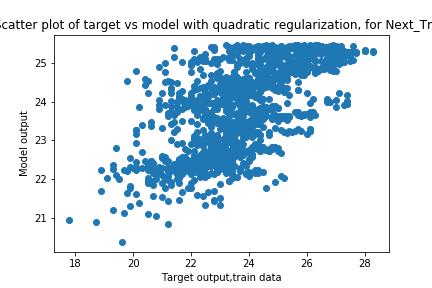
\includegraphics[scale=0.5]{images/scatter_ds3quadtrainT_min.png}
     \caption{Scatter plot of the target values vs model prediction for Training set of Dataset 3, using linear regression with gaussian basis and quaadratic Regularization, $\lambda = 0.01 $ for "NTmin" output variable}
     \label{fig:tikhds2tr}
\end{figure}
\begin{figure}[H]
     \centering
     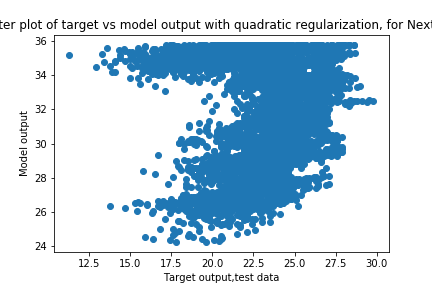
\includegraphics[scale=0.5]{images/scatter_ds3quadtestT_min.png}
     \caption{Scatter plot of the target values vs model prediction for Test set of Dataset 2, using linear regression with gaussian basis and quadratic Regularization, $\lambda = 0.01 $, for "NTmin" output variable}
     \label{fig:tikhds2tr}
\end{figure}
For "NTmax":
\begin{figure}[H]
     \centering
     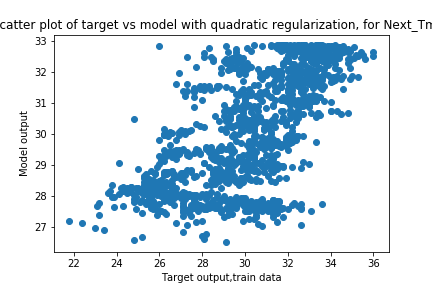
\includegraphics[scale=0.5]{images/scatter_ds3quadtrainT_max.png}
     \caption{Scatter plot of the target values vs model prediction for Training set of Dataset 3, using linear regression with gaussian basis and quaadratic Regularization, $\lambda = 0.01 $ for "NTmax" output variable}
     \label{fig:tikhds2tr}
\end{figure}
\begin{figure}[H]
     \centering
     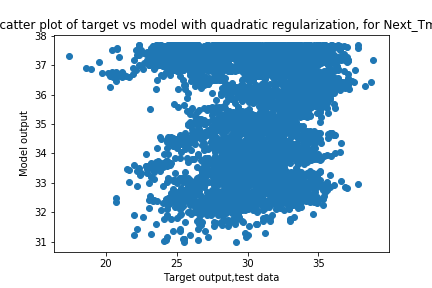
\includegraphics[scale=0.5]{images/scatter_ds3quadtestT_max.png}
     \caption{Scatter plot of the target values vs model prediction for Test set of Dataset 2, using linear regression with gaussian basis and quadratic Regularization, $\lambda = 0.01$, for "NTmax" output variable}
     \label{fig:tikhds2tr}
\end{figure}

\subsection{Tikhonov Regularization} 
The Tikhonov regularization term is given by $\vec{\omega^*}$ = $(\Phi*T\Phi + \lambda \Tilde{\Phi})^{-1} \Phi^T \vec{t}$. The $\Tilde{\Phi}$ term is defined as 
\begin{equation}
    \Tilde{\Phi} = [\Tilde{\phi}]_{i,j = 1}^{K}
\end{equation}

where K is the number of clusters and $\lambda$ is the regularization parameter. The values 0.01,0.1, 1.0,5.0,10.0 were used to estimate the optimal parameters and the RMSE on the cross-validation set was calculated for each value. The best perorming model was selected as the one having least RMSE on CV data\\ 
Applying Tikhonov regularization to the bivariate dataset, the optimal value of $\lambda$ was estimated to be 0.01. 
 The table for the RMSE values for the Training, CV and Test values corresponding to each $\lambda$ value is
\def\arraystretch{1.25}
\begin{table}[H]
\centering
\begin{tabular}{l l l l}
\hline
\hline
\textbf{Lambda} & \textbf{RMSE Train} & \textbf{RMSE CV} & \textbf{RMSE test} \\
\hline
\hline
0.01 & 78112040.25241715 & 80416219813.42682 & 43898825037.538 \\
0.1 & 78629878.58895023 & 276304216179.1798 & 176596027875.55765 \\
1.0 & 79471104.52781227 & 357583741029.9827 & 104372422450.83612 \\
5.0 & 77593937.82583737 & 272444591755.6569 & 174802698267.85687 \\
10.0 & 77693846.61754198 & 242869557997.72043 & 158196054705.92648 \\
\hline
\end{tabular}
\caption{Results obtained for Task 3}
\end{table}


\noi
Scatter plots of the model prediction using the regularization parameter value 0.01:
\begin{figure}[H]
     \centering
     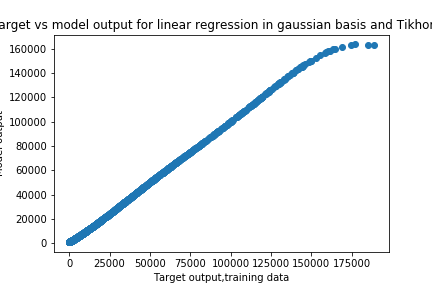
\includegraphics[scale=0.5]{images/scatter_ds2tikhtr.png}
     \caption{Scatter plot of the target values vs model prediction for Training set of Dataset 2, using linear regression with gaussian basis and Tikhonov Regularization, $\lambda = 0.01 $}
     \label{fig:tikhds2tr}
\end{figure}
\begin{figure}[H]
     \centering
     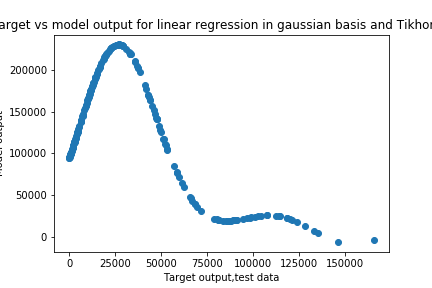
\includegraphics[scale=0.5]{images/scatter_ds2tikhtest.png}
     \caption{Scatter plot of the target values vs model prediction for Test set of Dataset 2, using linear regression with gaussian basis and Tikhonov Regularization, $\lambda = 0.01 $}
     \label{fig:tikhds2tr}
\end{figure}

 \noi
For Dataset 3, the table for the RMSE values for the Training, CV and Test values corresponding to each $\lambda$ value corresonding to target variable "NTmin" is\\
\def\arraystretch{1.25}
\begin{center}
\begin{longtable}{l l l l}
\hline
\hline
\textbf{Lambda} & \textbf{RMSE Train} & \textbf{RMSE CV} & \textbf{RMSE test} \\
\hline
\hline
0.01 & 4929.01653053444 & 414848.3042013735 & 3312196.0992440097 \\
0.1 & 4624.091536077471 & 1669.205290237633 & 36902.34473960538 \\
1.0 & 4637.926167783597 & 2073.9375316355663 & 39568.04405922714 \\
5.0 & 4652.374704231647 & 2257.2672544567195 & 40450.17809627787 \\
10.0 & 4667.40003673528 & 2346.920490034092 & 40853.959722564214 \\
\hline
\end{longtable}
\setcounter{table}{0}
\captionof{table}{Results obtained for Task 3}
\end{center}


\noi
the optimal value of $\lambda$ was estimated to be 0.1 for the target output "NTmin". The scatter plots obtained are Figures \ref{fig:tikhds3tr} and \ref{fig:tikhds3t}
\begin{figure}[H]
     \centering
     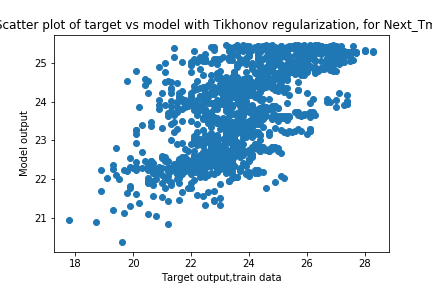
\includegraphics[scale=0.5]{images/scatter_ds3tikhtrainT_min.png}
     \caption{Scatter plot of the target values vs model prediction for Training set of Dataset 3, using linear regression with gaussian basis and Tikhonov Regularization, $\lambda = 0.1 $}
     \label{fig:tikhds3tr}
\end{figure}
\begin{figure}[H]
     \centering
     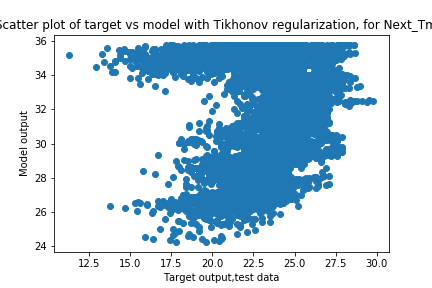
\includegraphics[scale=0.5]{images/scatter_ds3tikhtestT_min.png}
     \caption{Scatter plot of the target values vs model prediction for Test set of Dataset 3, using linear regression with gaussian basis and Tikhonov Regularization, $\lambda = 0.01 $}
     \label{fig:tikhds3t}
\end{figure}
 For the target output "NTmax" the following table of RMSE values for the training, test and CV data was obtained:
\def\arraystretch{1.25}
\begin{table}[H]
\centering
\begin{tabular}{l l l l}
\hline
\hline
\textbf{Lambda} & \textbf{RMSE Train} & \textbf{RMSE CV} & \textbf{RMSE test} \\
\hline
\hline
0.01 & 4929.01653053444 & 414848.3042013735 & 3312196.0992440097 \\
0.1 & 4624.091536077471 & 1669.205290237633 & 36902.34473960538 \\
1.0 & 4637.926167783597 & 2073.9375316355663 & 39568.04405922714 \\
5.0 & 4652.374704231647 & 2257.2672544567195 & 40450.17809627787 \\
10.0 & 4667.40003673528 & 2346.920490034092 & 40853.959722564214 \\
\hline
\end{tabular}
\caption{Results obtained for Task 3}
\end{table}

 plots were obtained: figures \ref{fig:tikhds3tr2} and \ref{fig:tikhds3t2}.
\begin{figure}[H]
     \centering
     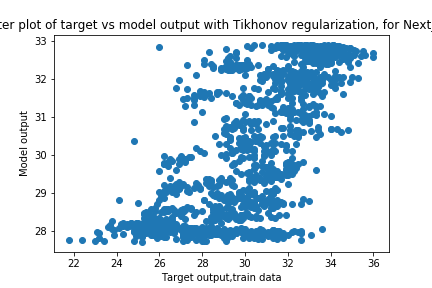
\includegraphics[scale=0.5]{images/scatter_ds3tikhtrainT_max.png}
     \caption{Scatter plot of the target values vs model prediction for Training set of Dataset 3, using linear regression with gaussian basis and Tikhonov Regularization, $\lambda = 0.1 $}
     \label{fig:tikhds3tr2}
\end{figure}
\begin{figure}[H]
     \centering
     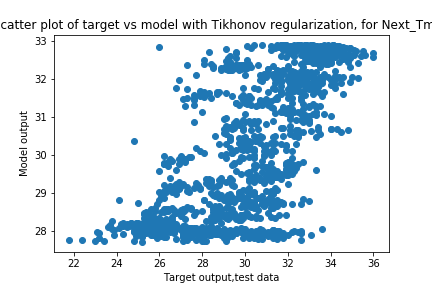
\includegraphics[scale=0.5]{images/scatter_ds3tikhtestT_max.png}
     \caption{Scatter plot of the target values vs model prediction for Test set of Dataset 3, using linear regression with gaussian basis and Tikhonov Regularization, $\lambda = 0.1 $}
     \label{fig:tikhds3t2}
\end{figure}

% \break
% \bibliographystyle{unsrt}
% \bibliography{reference}
\end{document}
